\subsection{Passage du modèle Entité-Association au modèle relationnel}
Nous avions pour consigne d'utiliser un schéma Entité-Association précis et de réaliser le modèle relationnel correspondant.

\begin{figure}[H]
	\begin{center}
	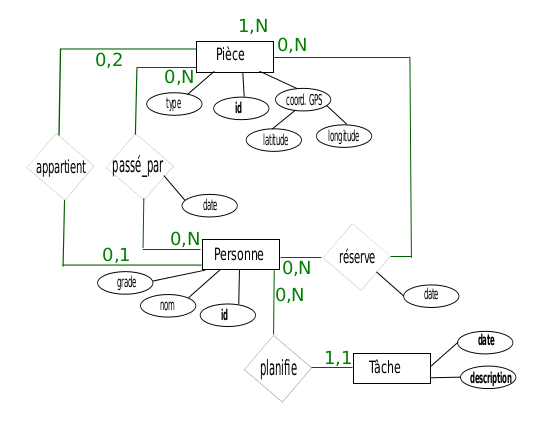
\includegraphics[width=350px]{./images/SchemaEA.png}
	\end{center}
\caption{Schéma EA}
\label{Schéma EA}
\end{figure}

En suivant chaque étape du cours, nous avons obtenu les résultats suivants :

\begin{enumerate}
	\item Passage des entités en relations :
		\begin{itemize}
			\item \code{piece}(idPiece, type, latitude, longitude) : l'attribut composite coord\_GPS est remplacé par ces 2 attributs, latitude et longitude.
			\item \code{personne}(id, nom, grade)
			\item \code{tache}(date, tache) 
		\end{itemize}
	\item Passage des entités faibles en relations : rien à faire puisqu'il n'y a pas d'entités faibles
	\item Association binaire 1,1 par clés étrangères :
		\begin{itemize}
			\item \code{piece}(idPiece, type, latitude, longitude) : schéma inchangé
			\item \code{personne}(id, nom, grade) : schéma inchangé
			\item \code{tache}(date, tache, id) : ajout de la clé étrangère id, clé de \code{personne} car il y a une cardinalité 1,1
		\end{itemize}
	\item Assocations binaires M,N :
		\begin{itemize}
			\item \code{piece}(idP, type, latitude, longitude) : schéma inchangé
			\item \code{personne}(idPers, nom, grade) : schéma inchangé
			\item \code{tache}(date, tache, idPers) : schéma inchangé
			\item \code{appartient}(idP, idPers) : création de la relation \code{appartient} à cette étape
			\item \code{passepar}(idP, idPers, date) : création de la relation \code{passepar} à cette étape
			\item \code{reservation}(idP, idPers, date) : création de la relation \code{reservation} à cette étape
		\end{itemize}
	\item Il n'y a pas d'attributs multi-valués ni d'association n-aire.
\end{enumerate}

\subsection{Critique du modèle proposé}